\subsection{Implementando Una Validación} \label{sec:validation}

% Teniendo definida la notación a usar para la declaración de las arquitecturas objetivo, lo siguiente a realizar era un módulo el cual se encargara de la validación, y construcción, los modelos a usar como referencia. 

Partiendo de la notación definida para la declaración de las arquitecturas de referencia, se realizó la implementación de un cliente que nos permitiera realizar la validación de los archivos de configuración.

Este cliente, apodado \textit{Lexical}, tiene como objetivo el tomar dichos archivos, y deserializarlos en las diferentes estructuras de datos definidas en el modelo, validando que estas cumplan con la sintaxis definida y que contengan los valores esperados. El grueso de este proceso se puede ver en la figura \ref*{fig:LexicalFlow}.

\begin{figure}[ht]
    \centering
    \caption{Diagrama de flujo del proceso realizado por el módulo \textit{Lexical}}
    \label{fig:LexicalFlow}
    \vspace{2mm}
    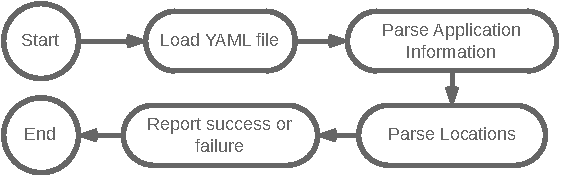
\includegraphics[width=0.75\linewidth]{images/LexicalFlow.pdf}
\end{figure}

Las 2 primeras partes del proceso son bastante directas. Lo primero es cargar el archivo indicado, validando que sea de tipo YAML; y tomar los datos del manifesto de la aplicación, en este caso el nombre y la descripción.

Seguido de esto, para la deserialización de las locaciones, se tendrán que recorrer cada una de las llaves presentes, procesando los valores internos de la locación. Como se estableció anteriormente, estas pueden ser, o más locaciones, hijas de la locación superior; o requerimientos de datos. El diagrama de dicho proceso se puede ver en la figura \ref{fig:LexicalLocations}.

\begin{figure}[ht]
    \centering
    \caption{Diagrama de flujo para validación y procesamiento de las locaciones}
    \label{fig:LexicalLocations}
    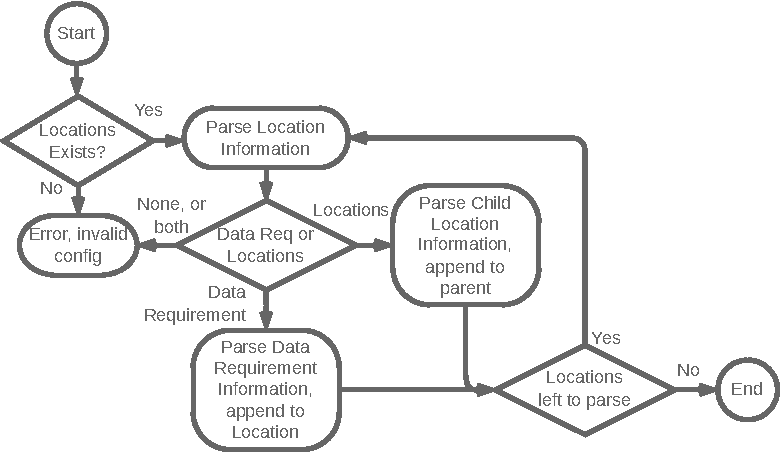
\includegraphics[width=\linewidth]{images/LexicalLocationsFlow.pdf}
\end{figure}


Este proceso de realiza para cada una de las locaciones registradas, lo que nos da como resultado el contexto geográfico en el que trabajaría la aplicación. Ahora, en cuanto al proceso de la validación de los requerimientos de datos, como se ve en la figura \ref{fig:LexicalDataReq}, es bastante directo en cuanto se toman las propiedades, definidas en el metamodelo; con la particularidad de crear un array vacío para los componentes. Esto se debe a que, en el momento de declarar la arquitectura, no conocemos ninguno de los datos necesarios para crearlos. Siendo así, estos se crearan durante la ejecución, a partir de los mensajes de los dispositivos.

\begin{figure}[ht]
    \centering
    \caption{Diagrama de flujo del procesamiento de los requerimientos de datos}
    \label{fig:LexicalDataReq}
    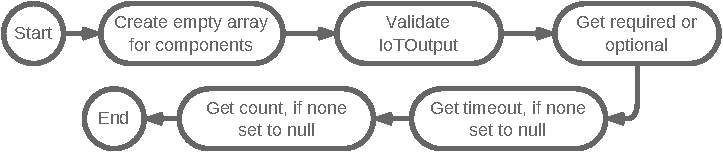
\includegraphics[width=0.9\linewidth]{images/LexicalDataRqeFlow.pdf}
\end{figure}

El desarrollo de este módulos, se realizó en Rust. Escogido debido a su capacidad para garantizar la integridad de los datos y prevenir errores comunes, lo que es esencial en un entorno donde la precisión y la confiabilidad son críticas. Además, su ecosistema de herramientas y bibliotecas facilita la implementación eficiente de los módulos de validación y construcción de modelos.\footnote{El código fuente de Lexical puede encontrase en el repositorio de GitHub: \url{https://github.com/ChipDepot/Lexical}}

Con la implementación de este módulo de validación, hemos completado la primera fase del desarrollo de una notación propia para describir y una herramienta para validar arquitecturas de aplicaciones de Smart Campus. Ahora podemos avanzar en la implementación de las funcionalidades de comparación y adaptación de modelos, que son parte fundamental del enfoque a computación autonómica. 


